% Manuel d'utilisation de l'extension Kab-board pour navigateur.
% Compilation : pdflatex manuel.tex, deux fois (sommaire et renvois).

\documentclass[11pt,a4paper]{article}

\usepackage[a4paper,margin=25mm]{geometry}
\usepackage{tipa}
\usepackage[T1]{fontenc}
\usepackage[utf8]{inputenc}
\usepackage{lmodern}
\usepackage{newunicodechar}
% Les lettres kabyles du texte.
\newunicodechar{ɣ}{\textipa{G}}
\newunicodechar{ɛ}{\textipa{E}}
\newunicodechar{ḍ}{\d{d}}
\newunicodechar{ḥ}{\d{h}}
\newunicodechar{ṭ}{\d{t}}
\newunicodechar{ẓ}{\d{z}}
\newunicodechar{ṣ}{\d{s}}
\newunicodechar{ṛ}{\d{r}}
\newunicodechar{ǧ}{\v{g}}
\newunicodechar{→}{\ensuremath{\rightarrow}}
\usepackage[french]{babel}
\frenchsetup{og=«, fg=», StandardItemLabels=true, SmallCapsFigTabCaptions=false}
\usepackage{microtype}
\usepackage{graphicx}
\graphicspath{{captures/}}
\usepackage{float}
\usepackage[section]{placeins}
\renewcommand{\topfraction}{0.85}
\renewcommand{\textfraction}{0.1}
\renewcommand{\floatpagefraction}{0.75}
\usepackage[font=small,labelfont=bf]{caption}
\usepackage{tabularx,booktabs,array}
\usepackage{amssymb}
\usepackage[hidelinks]{hyperref}
\hypersetup{pdftitle={Kab-board, extension pour navigateur : manuel d'utilisation},pdfauthor={Massil Aoudj},pdflang={fr}}

% Un bouton, une case ou un menu de Kab-board ou de Chrome.
\newcommand{\bouton}[1]{\textsf{#1}}
% Un mot kabyle cité.
\newcommand{\kab}[1]{\textit{#1}}
% Ce qu'on tape.
\newcommand{\touche}[1]{\texttt{#1}}
% Une adresse, un chemin, un fichier.
\newcommand{\chemin}[1]{\texttt{#1}}
\newcommand{\menu}{\enspace›\enspace}

% Une remarque : un titre en gras, puis le texte.
\newenvironment{encadre}[2][]{\par\medskip\noindent\textbf{#2.}\ }{\par\medskip}

% Une capture et sa légende.
\setlength{\fboxsep}{0pt}
\setlength{\fboxrule}{0.4pt}
\newcommand{\capture}[3][\dimexpr\linewidth-2\fboxrule\relax]{%
  \begin{figure}[!htb]
  \centering\fbox{\includegraphics[width=#1]{#2}}
  \caption{#3}\label{f:#2}
  \end{figure}}

\newcolumntype{L}{>{\raggedright\arraybackslash}X}
\newcommand{\tableau}[3]{%
  \par\noindent\begin{tabularx}{\linewidth}{@{}>{\raggedright\arraybackslash}p{#1}L@{}}
  \toprule #2 \\ \midrule #3 \bottomrule
  \end{tabularx}\par}

\title{Kab-board, extension pour navigateur\\[0.4em] \large Chrome, Edge, Brave, Opera : le clavier et le correcteur kabyles dans le navigateur. Manuel d'utilisation, version 0.2}
\author{}
\date{30 octobre 2026}

\begin{document}

\maketitle

\begin{abstract}
L'extension Kab-board apporte le clavier et le correcteur kabyles dans les navigateurs Chrome, Edge, Brave, Opera et Chromium : les lettres kabyles depuis votre clavier habituel, six propositions sous le mot, les fautes soulignées pendant que vous écrivez, la dictée en kabyle et les outils d'Asegzawal. Le but : écrire et corriger le kabyle là où l'on rédige du texte dans le navigateur, Microsoft 365 en ligne compris. Ce manuel en décrit l'installation et chaque fonction. Les captures sont faites dans Chrome ; dans Edge, Brave et Opera, tout se passe de la même façon. L'extension se suffit à elle-même : le correcteur, le modèle de langue et le modèle vocal de Kab-board sont dedans, et tournent dans le navigateur. Rien à installer à côté, et rien n'est envoyé sur Internet.
\end{abstract}

\capture[0.8\linewidth]{03-barre-correction.png}{Dans un champ de message : la barre des propositions sous le mot « ruhaɣ ».}

\noindent{\small Kab-board, clavier et correcteur kabyles. Licence GNU GPL version 3 ou ultérieure. Le lexique et le modèle de langue sont publiés sous licence CC BY-SA 4.0, doi 10.5281/zenodo.22112059. La dictée utilise le modèle vocal Mmeslay (Aomer Gaya Ouldali), sous licence GNU GPL version 3.}

% ---------------------------------------------------------------- Sommaire
\clearpage
\renewcommand{\contentsname}{Sommaire}
\setcounter{tocdepth}{1}
\tableofcontents
\clearpage

% ---------------------------------------------------------------- 1
\section{À quoi elle sert}\label{s:but}
Le but de l'extension : écrire et corriger le kabyle \textbf{là où l'on rédige du texte} dans le navigateur : les zones de texte des messages, des documents, des publications et des formulaires. Elle marche notamment dans \textbf{Microsoft 365 en ligne}, par exemple dans Word ouvert dans le navigateur, où le complément Kab-board pour Word ne peut pas s'installer. Elle marche aussi dans les messageries (WhatsApp Web…), les réseaux sociaux et les formulaires.

\begin{encadre}{Tout est dans l'extension}
Le correcteur de Kab-board pour Android (1,58 million de formes, un modèle de langue, un modèle vocal) est dans l'extension et tourne dans le navigateur, sur l'ordinateur. Il donne les mêmes propositions, les mêmes soulignés et la même dictée que l'application Android. Rien ne passe par Internet.
\end{encadre}

% ---------------------------------------------------------------- 2
\section{Guide d'installation}\label{s:installer}
Il faut un navigateur récent : Google Chrome 116 ou plus récent, Microsoft Edge, Brave, Opera ou Chromium, sous Windows, macOS ou Linux. Rien d'autre à installer.

\subsection{Télécharger l'extension}
L'extension se télécharge avec les autres versions de Kab-board, sur la page des versions du dépôt : \url{https://github.com/ADJ-MSS/kab-board/releases}. C'est le fichier \chemin{kab-board-navigateur-0.2.0.zip}, d'environ 245~Mo : le correcteur, le modèle de langue et le modèle vocal sont dedans.

\subsection{L'ajouter au navigateur, en mode développeur}
\begin{enumerate}
  \item \textbf{Décompressez} l'archive dans un dossier où elle restera, par exemple vos Documents.
  \item \textbf{Ouvrez} \chemin{chrome://extensions} dans la barre d'adresse (\chemin{edge://extensions} dans Edge, \chemin{brave://extensions} dans Brave, \chemin{opera://extensions} dans Opera).
  \item \textbf{Allumez} \bouton{Mode développeur}, en haut à droite.
  \item \textbf{Cliquez sur} \bouton{Charger l'extension non empaquetée} et choisissez le dossier décompressé, celui qui contient \chemin{manifest.json}.
\end{enumerate}

\capture{01-extensions.png}{L'extension chargée en mode développeur : Kab-board 0.2.0, allumée.}

\begin{encadre}{Pourquoi le mode développeur}
Kab-board n'est pas encore sur le Chrome Web Store, et hors du Web Store, Chrome n'installe une extension que de cette façon. Laissez son dossier là où il est : Chrome le relit à chaque démarrage. Si vous le déplacez, chargez-la de nouveau depuis sa nouvelle place.
\end{encadre}

\FloatBarrier
\subsection{Épingler le bouton}
Cliquez sur l'icône en forme de pièce de puzzle, à droite de la barre d'adresse, puis sur la punaise à côté de Kab-board. Son bouton reste alors visible : il donne les réglages et les outils (section~\ref{s:bouton}).

\subsection{La première fois}
À l'ajout de l'extension, sa page de réglages s'ouvre. En haut, « Prêt, sur cet ordinateur » dit que tout est en place. Le correcteur se prépare au premier champ où vous écrivez, en cinq secondes environ ; la frappe des lettres kabyles marche déjà pendant ce temps. Les onglets déjà ouverts n'ont pas besoin d'être rechargés.

% ---------------------------------------------------------------- 3
\section{Écrire les lettres kabyles}\label{s:lettres}
Cliquez dans n'importe quel champ d'une page et tapez comme on parle : Kab-board écrit la lettre kabyle à la place des deux lettres tapées l'une après l'autre. AltGr donne aussi les lettres directement.

\medskip
\tableau{0.24\linewidth}{\textbf{Vous tapez} & \textbf{Kab-board écrit}}{%
\touche{gh} & ɣ \\
\touche{dh} & ḍ \\
\touche{kh} & x \\
\touche{aa} & ɛ \\
\touche{ou} & u \\
AltGr + \touche{g}, \touche{e} & ɣ, ɛ \\
AltGr + \touche{d}, \touche{h}, \touche{t}, \touche{z}, \touche{s} & ḍ, ḥ, ṭ, ẓ, ṣ \\
AltGr + \touche{c}, \touche{j}, \touche{r} & č, ǧ, ṛ \\}

\medskip
Un effacement juste après une conversion la défait : \touche{gh} redevient \touche{gh}, pour l'écrire pour de bon. \touche{Ctrl+Z} la défait aussi, comme toute frappe. Sur un clavier sans touche AltGr, les paires de lettres suffisent.

% ---------------------------------------------------------------- 4
\section{La barre des propositions}\label{s:barre}
Pendant que vous tapez un mot, une petite barre s'ouvre juste sous lui, avec six propositions, à la casse du mot tapé. Le trait sous chacune dit ce qu'elle est :

\medskip
\tableau{0.14\linewidth}{\textbf{Couleur} & \textbf{Ce que c'est}}{%
vert & La correction en contexte : ce que le correcteur choisirait, compte tenu des mots d'avant. \\
bleu & Les autres candidats pour ce mot. \\
ocre & De 1 à 3 lettres, les mots qui commencent ainsi ; le mot fini, ceux qui viennent souvent après. \\}

\capture[0.8\linewidth]{04-barre-completion.png}{Trois lettres : les mots qui commencent par « tam ».}
\capture[0.8\linewidth]{05-barre-prediction.png}{Le mot fini : la suite probable, en ocre.}

\begin{encadre}{Rien n'est corrigé d'office}
L'espace écrit le mot tel que vous l'avez tapé. Les propositions ne s'écrivent que si vous les choisissez. Au bout de la barre, le micro lance la dictée (section~\ref{s:dicter}) et le logo de Kab-board ouvre les outils (section~\ref{s:outils}).
\end{encadre}

\FloatBarrier
\subsection{Choisir une proposition}
\begin{itemize}
  \item un clic sur la proposition ;
  \item ou un chiffre de \touche{1} à \touche{6} : 1 pour la première, 2 pour la deuxième, et ainsi de suite. En AZERTY, les chiffres se tapent avec Maj, ou au pavé numérique ;
  \item \touche{Échap} cache la barre sans rien écrire.
\end{itemize}
La proposition remplace le mot tapé, suivie d'une espace s'il n'y en a pas déjà une. Au milieu d'un mot, la barre propose pour ce qui précède le curseur, et la proposition remplace le mot entier. Les chiffres ne choisissent que pendant qu'un mot s'écrit : après une espace, ils s'écrivent normalement.

\FloatBarrier
\subsection{Les possessifs : « tamurt iw » → « tamurt-iw »}
Un possessif (\kab{iw}, \kab{ik}, \kab{im}, \kab{is}, \kab{nneɣ}, \kab{nwen}\dots) s'attache au mot d'avant par un tiret. Tapez-le comme un mot à part : la barre propose les deux mots rattachés, en tête, et les écrit en une fois. Jamais par-dessus une virgule.
\capture[0.8\linewidth]{06-barre-possessif.png}{« tamurt iw » : « tamurt-iw » en tête, en vert.}
\capture[0.8\linewidth]{07-possessif-choisi.png}{Choisi : les deux mots n'en font qu'un, et la barre propose la suite.}

% ---------------------------------------------------------------- 5
\section{Les mots soulignés}\label{s:soulignes}
Pendant que vous écrivez, Kab-board relit la phrase où vous êtes et souligne les mots à revoir :
\begin{itemize}
  \item \textbf{en rouge}, un mot que le correcteur ne connaît pas : une faute probable ;
  \item \textbf{en bleu}, un mot qu'il connaît, mais que la phrase écrirait autrement : un doute.
\end{itemize}
« tamurt iw » se souligne d'un seul tenant. Le mot que vous êtes en train de taper n'est pas souligné avant d'être fini. Le correcteur de Chrome, qui ne connaît pas le kabyle et soulignerait chaque mot, se tait dans le champ ; il revient si vous éteignez Kab-board.
\capture[0.8\linewidth]{08-soulignes.png}{Les mots à revoir : en bleu les doutes, en rouge « tamurt iw », à écrire en un seul mot.}

\FloatBarrier
\subsection{La carte d'un mot}
Un clic sur un mot souligné ouvre sa carte :
\begin{itemize}
  \item les propositions : un clic remplace le mot ;
  \item \bouton{Garder mon mot} : le mot reste tel quel et n'est plus souligné ;
  \item \bouton{Ajouter à mon dictionnaire} : il ne sera plus jamais souligné (section~\ref{s:dictionnaire}) ;
  \item \bouton{Asegzawal} : la fiche du mot.
\end{itemize}
\capture[0.8\linewidth]{09-carte.png}{La carte de « tamettut » : dans ce contexte, plutôt « tmeṭṭut ».}

\FloatBarrier
\subsection{Dans les éditeurs riches}
Kab-board écrit et souligne aussi dans les éditeurs de texte des sites (messageries, réseaux sociaux, outils de rédaction), sans toucher au texte : les soulignés sont dessinés par le navigateur, et \touche{Ctrl+Z} défait ce que Kab-board a écrit.
\capture[0.8\linewidth]{10-editable.png}{Dans un éditeur riche : les mêmes soulignés.}

% ---------------------------------------------------------------- 6
\section{La correction automatique, si vous le voulez}\label{s:auto}
Elle est éteinte au départ. Allumée (bouton Kab-board\menu\bouton{Réglages de l'écriture}\menu\bouton{Correction automatique}), elle corrige à l'espace un mot que le correcteur ne connaît pas, par sa correction en contexte. Elle ne touche jamais à un mot connu, à un nom propre au milieu d'une phrase, à un sigle, à un mot de « mon dictionnaire » ni à un mot que vous avez gardé. Juste après, \touche{Retour arrière} rend le mot que vous aviez tapé.

% ---------------------------------------------------------------- 7
\section{Le bouton Kab-board}\label{s:bouton}
Le bouton de l'extension, à droite de la barre d'adresse, ouvre ce panneau :
\begin{itemize}
  \item \bouton{Clavier kabyle} : l'allumer ou l'éteindre partout (\touche{Alt+Maj+K}) ;
  \item \bouton{Sur} \emph{ce site} : l'éteindre seulement sur le site ouvert ;
  \item \bouton{Graphie} v ou b (section~\ref{s:graphie}) ;
  \item \bouton{Dicter}, \bouton{Relire le champ}, les lettres kabyles à cliquer, \bouton{Écrire et relire} ;
  \item Asegzawal et la recherche du français au kabyle ;
  \item le mot du jour, qu'un clic sur \bouton{Copier} met dans le presse-papiers ;
  \item \bouton{Réglages de l'écriture}, et en bas \bouton{Tous les réglages, mon dictionnaire}.
\end{itemize}

\begin{figure}[!htb]
\centering
\fbox{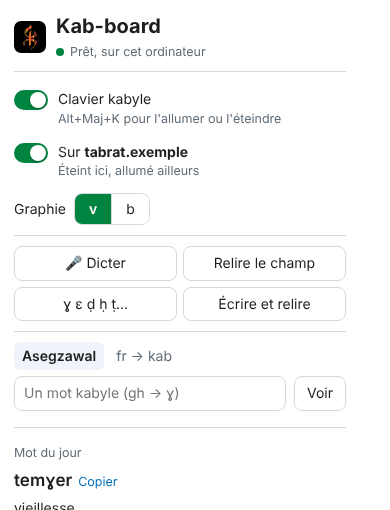
\includegraphics[width=0.42\linewidth]{19-popup.png}}\hfill
\fbox{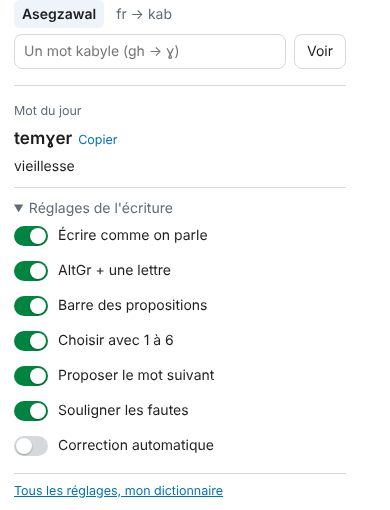
\includegraphics[width=0.42\linewidth]{20-popup-reglages.png}}
\caption{Le bouton Kab-board : en haut du panneau, et plus bas, les réglages de l'écriture.}\label{f:popup}
\end{figure}

Dans \bouton{Réglages de l'écriture}, chaque fonction s'allume ou s'éteint : écrire comme on parle, AltGr + une lettre, la barre des propositions, le choix avec 1 à 6, la proposition du mot suivant, les fautes soulignées, la correction automatique.

\capture[0.42\linewidth]{21-popup-asegzawal.png}{Asegzawal dans le panneau : la fiche de « aɣrum ». On tape « aghrum », gh devient ɣ.}

% ---------------------------------------------------------------- 8
\section{Les outils dans la page}\label{s:outils}
Le logo de Kab-board, au bout de la barre des propositions, ouvre les outils sans quitter le champ où vous écrivez. Ils ne prennent jamais le curseur : ce qu'ils écrivent va au curseur du champ.
\capture[0.8\linewidth]{11-outils.png}{Les outils : Dicter, Asegzawal, du français au kabyle, Relire, le mot du jour, les lettres kabyles, Écrire et relire, Réglages.}

\subsection{Asegzawal : la fiche d'un mot}
Le sens du mot sous le curseur, sa catégorie, et ses états libre et d'annexion quand le lexique les connaît.
\capture[0.8\linewidth]{12-asegzawal.png}{La fiche de « aɣrum » : pain, galette.}

\FloatBarrier
\subsection{Du français au kabyle}
Tapez un mot français : les mots kabyles qui le traduisent, avec leur sens.
\capture[0.8\linewidth]{13-fr-kab.png}{« pain » : aɣrum, iɣerman, lxebz\dots}

\FloatBarrier
\subsection{Le mot du jour, les lettres kabyles}
Le mot du jour est le même pour tout le monde, chaque jour : \bouton{Insérer} l'écrit au curseur. Les lettres kabyles s'écrivent d'un clic, en majuscules avec \bouton{Majuscules}.
\begin{figure}[!htb]
\centering
\fbox{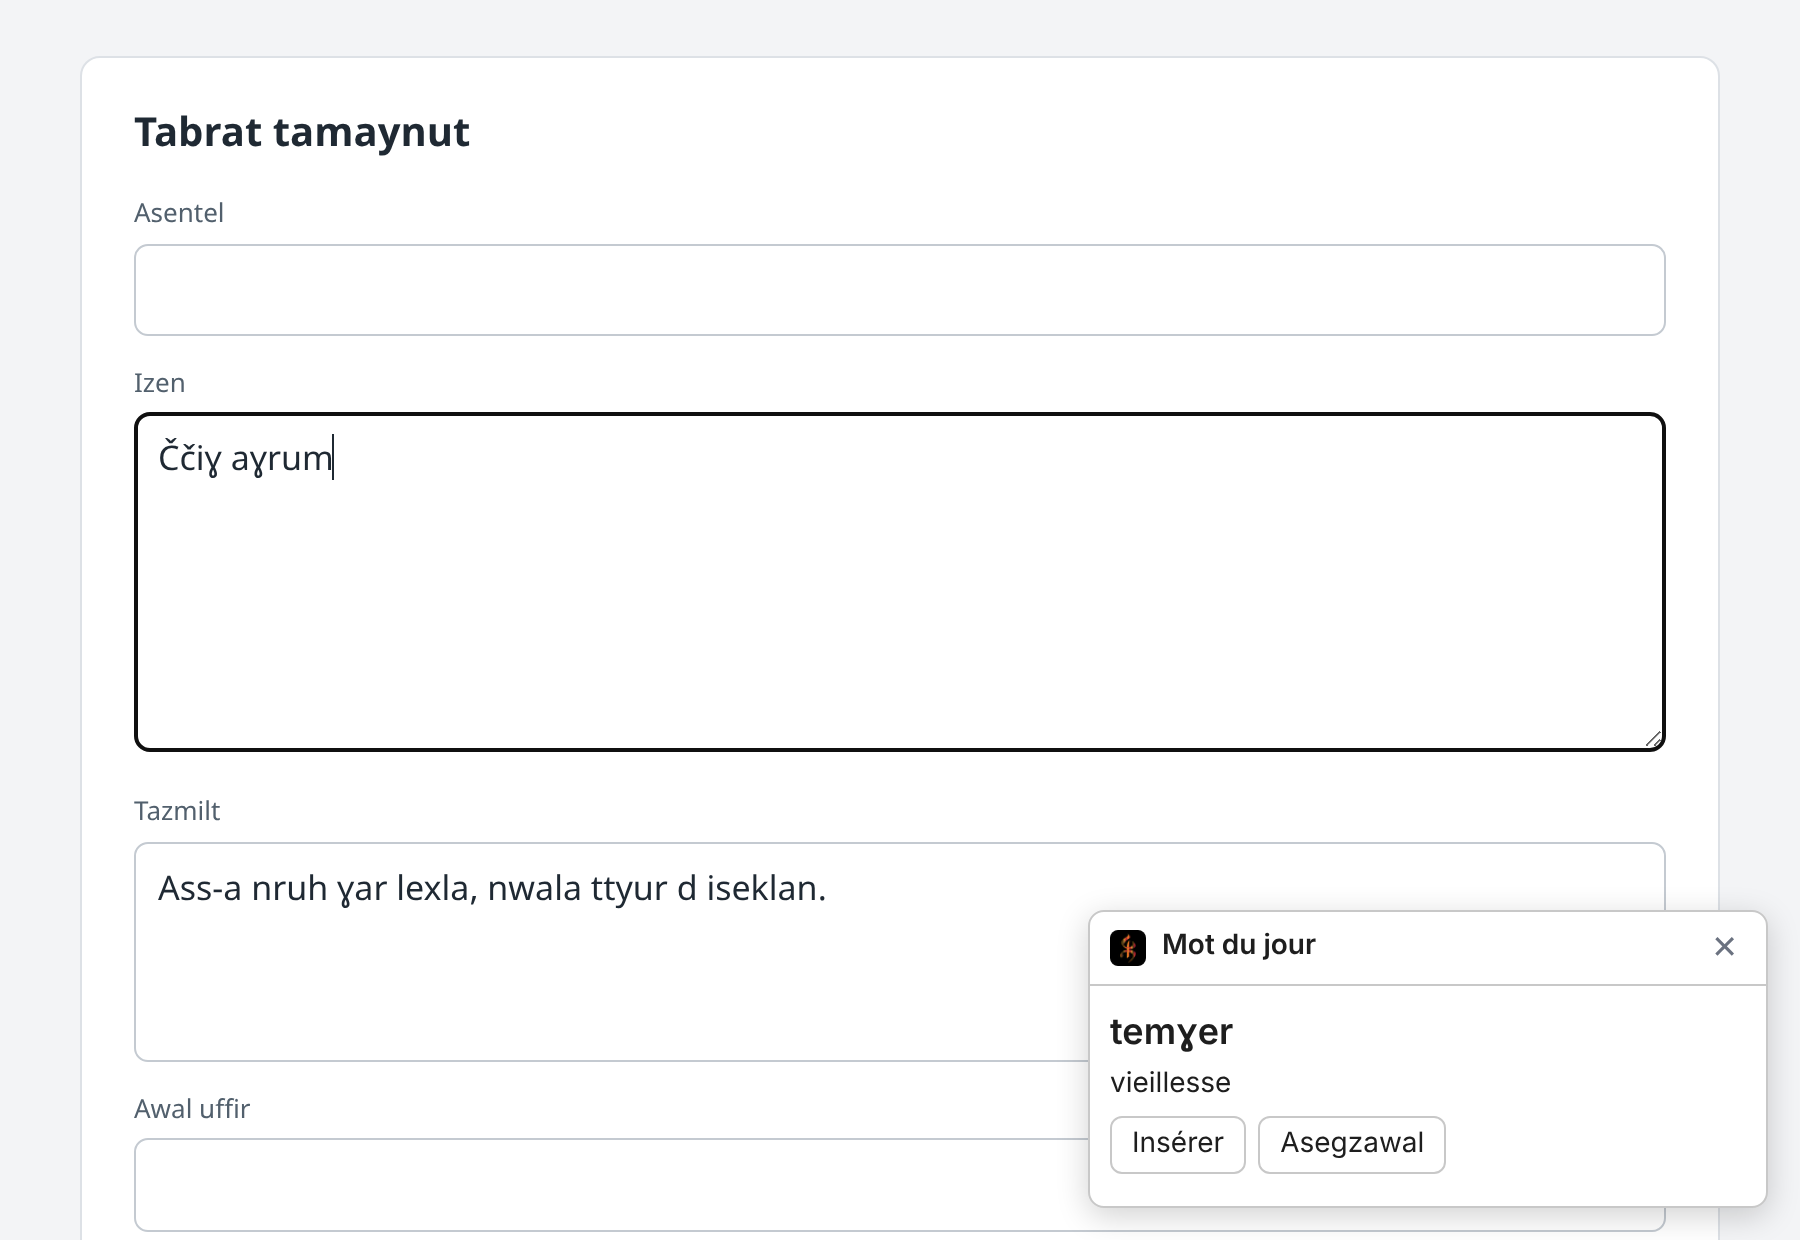
\includegraphics[width=0.48\linewidth]{14-mot-du-jour.png}}\hfill
\fbox{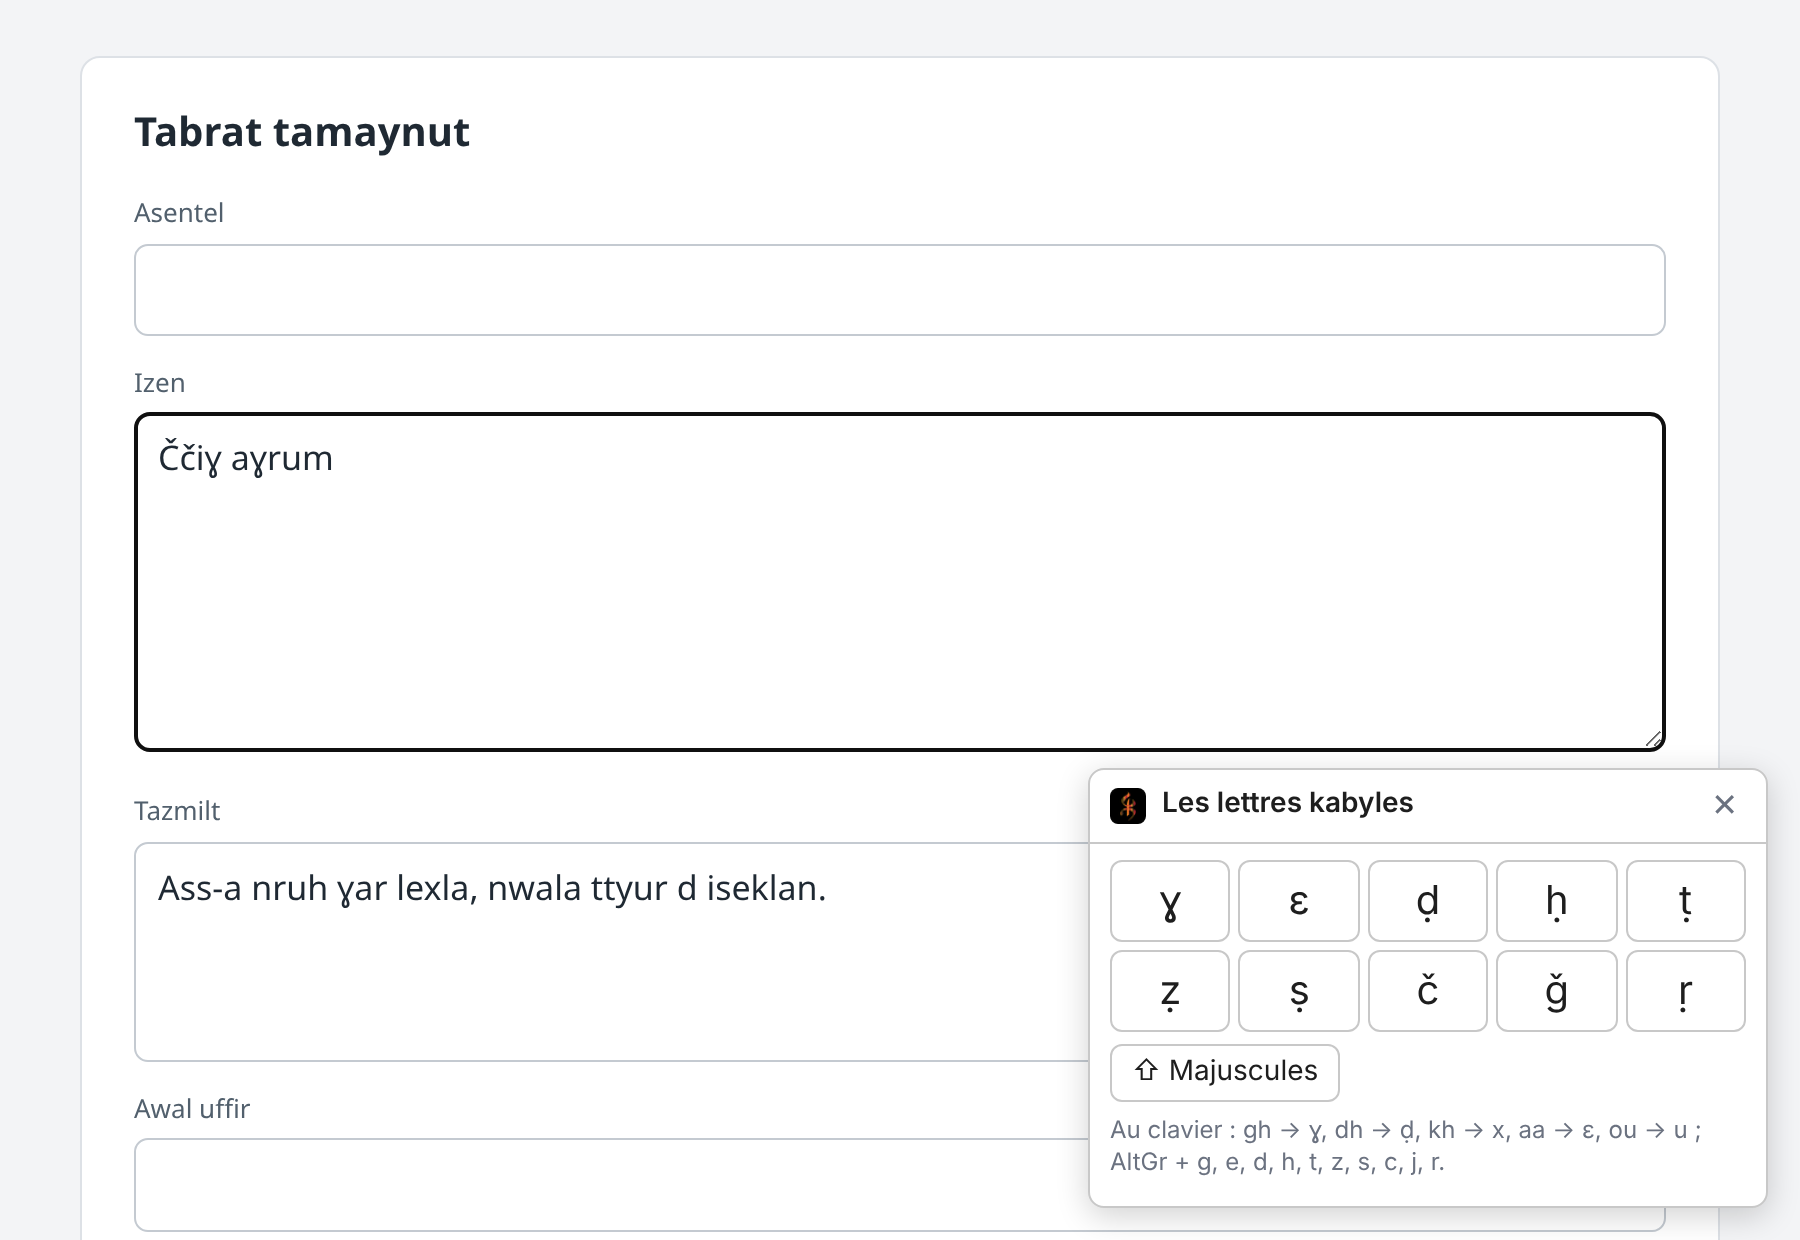
\includegraphics[width=0.48\linewidth]{15-lettres.png}}
\caption{Le mot du jour, et les lettres kabyles à cliquer.}\label{f:jour-lettres}
\end{figure}

\FloatBarrier
\subsection{Relire un champ, et tout corriger}
\bouton{Relire} (ou \touche{Alt+Maj+R}) liste les mots à revoir du champ, chacun avec quatre propositions au plus, \bouton{Garder}, \bouton{Ajouter à mon dictionnaire} et \bouton{Asegzawal}. \bouton{Tout corriger} remplace chaque mot par sa première proposition. Si du texte est sélectionné, seule la sélection est relue.
\capture[0.8\linewidth]{16-relire.png}{Relire : 5 mots à revoir, et « Tout corriger ».}

\FloatBarrier
\subsection{Le clic droit}
Sur une sélection ou dans un champ, le clic droit propose \bouton{Relire avec Kab-board}, \bouton{Dicter en kabyle}, \bouton{Asegzawal : «~…~»} et \bouton{Du français au kabyle : «~…~»}. Il marche aussi sur un texte que l'on ne peut pas modifier, dans une page.

% ---------------------------------------------------------------- 9
\section{Dicter en kabyle}\label{s:dicter}
\begin{enumerate}
  \item Cliquez dans le champ, puis sur le micro au bout de la barre (ou \touche{Alt+Maj+D}).
  \item Parlez en kabyle.
  \item Cliquez sur \bouton{Arrêter} (ou de nouveau \touche{Alt+Maj+D}) : le texte s'écrit au curseur, 30 secondes au plus.
\end{enumerate}
La toute première fois, Chrome demande l'accès au micro dans un onglet : cliquez sur \bouton{Autoriser le micro}, puis acceptez quand Chrome le demande.
\capture[0.6\linewidth]{24-micro.png}{L'onglet qui demande le micro, une seule fois.}
\capture[0.65\linewidth]{17-dictee.png}{La dictée écoute : « J'écoute\dots », et le bouton Arrêter.}
\capture[0.65\linewidth]{18-dictee-finie.png}{Le texte dicté, écrit au curseur : « ilaq ad teččem kra n lḥaǧa ».}

Le texte dicté n'est jamais corrigé d'office : les mots à revoir se soulignent, et \bouton{Relire la dictée} les liste. La voix est transcrite dans le navigateur, par le modèle vocal de Kab-board, et n'est gardée que le temps de la transcrire : elle n'est écrite nulle part.

% ---------------------------------------------------------------- 10
\section{La page « Écrire et relire »}\label{s:ecrire}
Certaines pages ne laissent écrire aucune extension : Google Docs, qui dessine son texte lui-même, les pages de Chrome, le Chrome Web Store. Pour elles, \bouton{Écrire et relire} (dans le bouton Kab-board ou les outils) ouvre une page où tout Kab-board marche : écrivez, relisez, puis \bouton{Copier le texte} et collez-le où vous voulez. Le texte est gardé dans le navigateur, sur cet ordinateur, jusqu'à ce que vous l'effaciez.
\capture[0.8\linewidth]{23-ecrire-relire.png}{« Écrire et relire » : la barre, les soulignés, et les outils en haut.}

% ---------------------------------------------------------------- 11
\section{Écrire avec v ou avec b}\label{s:graphie}
Certains écrivent \kab{avrid}, d'autres \kab{abrid}. Choisissez dans le bouton Kab-board ou les réglages. Le réglage vaut pour tout : les propositions, la prédiction, la fiche, la recherche, le mot du jour et la dictée. Au départ, c'est v, comme sur le téléphone. Il est gardé avec les autres réglages de l'extension, et vous suit sur vos autres ordinateurs si la synchronisation de Chrome est allumée.
\capture[0.8\linewidth]{25-graphie-b.png}{En graphie b, la prédiction propose « tbeddel » (« tveddel » en graphie v, figure~\ref{f:05-barre-prediction.png}).}

% ---------------------------------------------------------------- 12
\section{Les réglages}\label{s:reglages}
Bouton Kab-board\menu\bouton{Tous les réglages, mon dictionnaire} ouvre la page des réglages :
\begin{itemize}
  \item le clavier kabyle, la graphie et chaque fonction de l'écriture, comme dans le bouton ;
  \item mon dictionnaire (section~\ref{s:dictionnaire}) ;
  \item les sites où Kab-board se tait ;
  \item les raccourcis (section~\ref{s:raccourcis}) ;
  \item ce que devient ce que vous écrivez (section~\ref{s:donnees}).
\end{itemize}
\capture[0.75\linewidth]{22-reglages.png}{La page des réglages.}

\FloatBarrier
\subsection{Mon dictionnaire}\label{s:dictionnaire}
Les mots que Kab-board ne souligne jamais : des noms propres, des mots rares, des mots de votre parler. Ajoutez-les dans la page des réglages, ou depuis la carte d'un mot souligné. Ils sont gardés dans Chrome, sur cet ordinateur. \bouton{Importer un fichier\dots} ajoute d'un coup les mots d'un fichier texte, un par ligne : celui de Kab-board pour Windows, par exemple (\chemin{mots-a-moi.txt}). \bouton{Exporter} en fait un fichier, à garder ou à importer ailleurs.

\subsection{Les sites où Kab-board se tait}
Tapez l'adresse d'un site (par exemple \chemin{exemple.com}) puis \bouton{Ajouter} : Kab-board ne fait plus rien sur ce site. Le bouton Kab-board\menu\bouton{Sur} \emph{ce site} fait la même chose pour le site ouvert.

\subsection{Les raccourcis}\label{s:raccourcis}
\medskip
\tableau{0.22\linewidth}{\textbf{Raccourci} & \textbf{Ce qu'il fait}}{%
\touche{Alt+Maj+K} & allumer ou éteindre le clavier kabyle \\
\touche{Alt+Maj+D} & dicter dans le champ où l'on écrit ; encore une fois pour arrêter \\
\touche{Alt+Maj+R} & relire le champ où l'on écrit \\
\touche{1} à \touche{6} & choisir une proposition de la barre \\
\touche{Échap} & cacher la barre \\}

\medskip
Chrome peut laisser un raccourci sans touche, quand il en utilise déjà la combinaison : c'est arrivé à \touche{Alt+Maj+R} lors de nos essais. \bouton{Changer les raccourcis}, dans les réglages, ouvre \chemin{chrome://extensions/shortcuts}, où l'on en choisit un autre.
\capture[0.9\linewidth]{02-raccourcis.png}{Les raccourcis de Kab-board dans Chrome : le crayon en change un.}

% ---------------------------------------------------------------- 13
\section{Où Kab-board se tait}\label{s:tait}
\begin{itemize}
  \item Dans un \textbf{mot de passe}, même rendu visible, un code à usage unique, un numéro de carte, un champ d'adresse électronique : ni conversion, ni barre, ni souligné. Ces champs ne sont jamais lus.
  \item Dans la barre d'adresse de Chrome, où l'on tape une adresse ou une recherche : aucune extension n'y a accès.
  \item Dans les éditeurs de code des sites (CodeMirror, Monaco, Ace).
  \item Dans Google Docs, les pages de Chrome et le Chrome Web Store, où aucune extension ne peut écrire : utilisez « Écrire et relire » (section~\ref{s:ecrire}).
  \item Sur les sites que vous avez choisis, et partout quand le clavier kabyle est éteint.
\end{itemize}

% ---------------------------------------------------------------- 14
\section{Vos données}\label{s:donnees}
Ce que vous écrivez ne quitte pas l'ordinateur. Le correcteur et le modèle vocal sont dans l'extension, qui n'ouvre aucune connexion vers Internet : tout se calcule dans le navigateur. La voix de la dictée n'est gardée que le temps de la transcrire, en mémoire. Les mots de passe, les codes et les numéros de carte ne sont jamais lus.

\medskip
\tableau{0.3\linewidth}{\textbf{Ce que l'extension demande} & \textbf{Pour quoi faire}}{%
stockage & garder vos réglages et « mon dictionnaire » \\
menus contextuels & le clic droit \\
document hors écran & le correcteur, chargé une fois pour tous les onglets, et le micro pendant la dictée \\
accès aux sites & écrire et souligner dans les champs des pages, y compris dans les onglets déjà ouverts \\}

\medskip
Le correcteur ne se charge qu'au premier champ où vous écrivez, en cinq secondes environ, et occupe alors à peu près 750~Mo de mémoire. Au bout de vingt minutes sans rien lui demander, il se libère, et se recharge au champ suivant.

% ---------------------------------------------------------------- 15
\section{Si le correcteur ne se charge pas}\label{s:panne}
Sur un ordinateur qui manque de mémoire, le correcteur peut ne pas se charger. L'extension écrit encore les lettres kabyles, mais ne propose ni ne corrige rien. Elle le dit une fois dans la page, son bouton le dit, et l'icône de l'extension porte un « ! ».
\begin{figure}[!htb]
\centering
\fbox{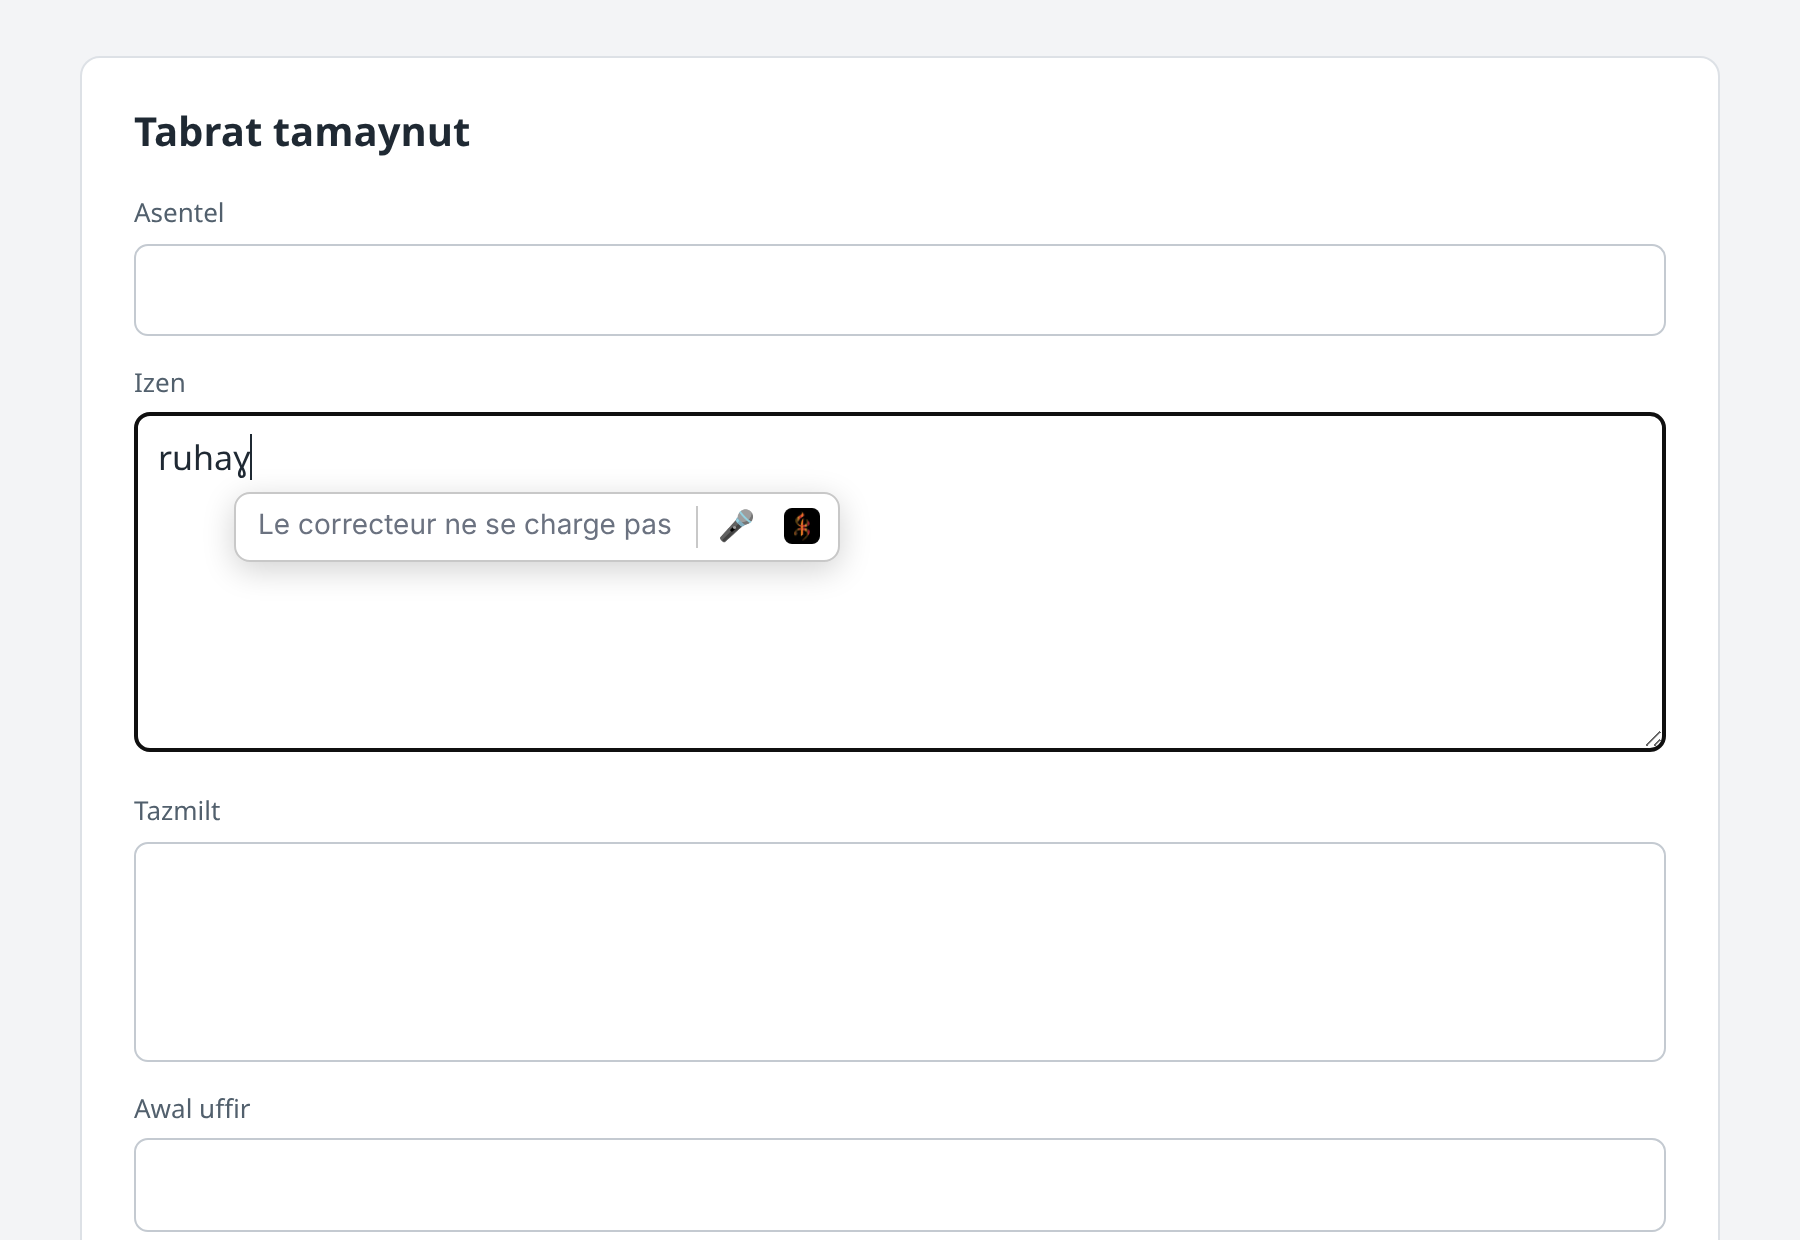
\includegraphics[width=0.5\linewidth]{27-panne-site.png}}\hfill
\fbox{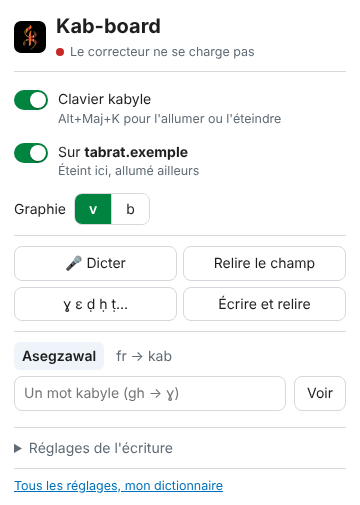
\includegraphics[width=0.42\linewidth]{28-panne-popup.png}}
\caption{Le correcteur ne se charge pas : « ruhagh » devient bien « ruhaɣ », mais sans propositions ; la page et le bouton le disent.}\label{f:panne}
\end{figure}

Fermez quelques onglets, puis, dans les réglages de l'extension, cliquez sur \bouton{Réessayer}. Ouvrir le bouton Kab-board ou les réglages le recharge aussi.
\capture[0.75\linewidth]{26-panne-reglages.png}{La page des réglages, quand le correcteur ne se charge pas.}

% ---------------------------------------------------------------- 16
\section{Retirer l'extension}\label{s:retirer}
\chemin{chrome://extensions}, puis \bouton{Supprimer} sur la carte de Kab-board (ou un clic droit sur son bouton, puis \bouton{Supprimer de Chrome}). Vos réglages et « mon dictionnaire » partent avec elle : exportez d'abord votre dictionnaire si vous voulez le garder (section~\ref{s:dictionnaire}).

% ---------------------------------------------------------------- 17
\section{En cas de souci}\label{s:souci}
\medskip
\tableau{0.36\linewidth}{\textbf{Ce que vous voyez} & \textbf{Que faire}}{%
« Le correcteur ne se charge pas » & Fermez quelques onglets, puis \bouton{Réessayer} dans les réglages de l'extension (section~\ref{s:panne}). \\
Pas de barre sous le mot & Le correcteur se prépare : attendez quelques secondes. Vérifiez aussi que le clavier kabyle est allumé, sur ce site aussi, et que \bouton{Barre des propositions} est cochée. \\
Rien ne se passe dans une page & C'est peut-être un mot de passe, un éditeur de code, Google Docs ou une page de Chrome : utilisez « Écrire et relire ». \\
La touche 1 écrit « \& » & Clavier AZERTY : Maj + \touche{\&}, ou le pavé numérique. \\
« gh » s'écrit ɣ alors que je voulais gh & Effacez une fois juste après : « gh » revient. \\
La dictée dit qu'elle n'a pas le micro & Autorisez le micro dans l'onglet qui s'ouvre, ou dans les paramètres du site de Chrome. \\
\touche{Alt+Maj+R} ne fait rien & Chrome ne lui a pas donné de touche : choisissez-en une dans \chemin{chrome://extensions/shortcuts}. \\
L'extension chargée en mode développeur a disparu après une mise à jour du dossier & Rechargez-la (flèche ronde sur sa carte, dans \chemin{chrome://extensions}). \\}

\medskip
Pour signaler un problème : \url{https://github.com/ADJ-MSS/kab-board}.

\end{document}
